\documentclass[12pt]{article}
\usepackage[a4paper]{geometry}
\usepackage{fullpage}
\usepackage[T1]{fontenc}
\usepackage[utf8]{inputenc}
\usepackage{graphicx}
\usepackage{mathpazo}
\pagenumbering{gobble}
\usepackage{siunitx}
\sisetup{output-decimal-marker = {,}}
\usepackage{amsmath}
\usepackage{esdiff}
\usepackage[spanish]{babel}
\usepackage{steinmetz}
\usepackage{pdfpages}

\begin{document}

\title{\textsc{Teoría de Circuitos II} :: Primer parcial}

\date{27 de marzo de  2019}

\maketitle

\subsection*{Instrucciones}
\begin{itemize}
\item El examen tiene una duración de 90 minutos.
\item Cada problema se deberá entregar en hojas separadas.
\item No se permite el uso de documentación ni de calculadoras con capacidad de almacenamiento.
\item Las calificaciones se publicarán el día 5 de abril. La
  revisión del examen se realizará en el horario de tutoría de cada
  profesor durante la semana del 8 de abril.

\end{itemize}

\clearpage

\section{Elementos activos}

\begin{minipage}{0.5\textwidth}

  Determina el generador equivalente del circuito entre A y B modificando la geometría del circuito mediante movilidad y transformación de fuentes. Dibuja los circuitos correspondientes a cada paso de la modificación.

  Datos:

  $I_{g1} = I_{g2} = \SI{10}{\ampere}$

  $R_{i}= \SI{1}{\ohm}$%
\end{minipage}
\begin{minipage}{0.5\textwidth}
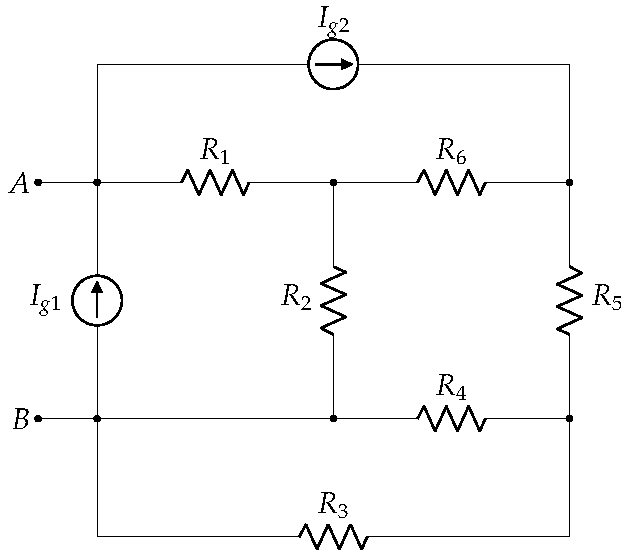
\includegraphics[width=\textwidth]{figs/movilidad.pdf}
\end{minipage}

\subsection*{Solución}

En primer lugar movemos la fuente $I_{g1}$:

\begin{center}
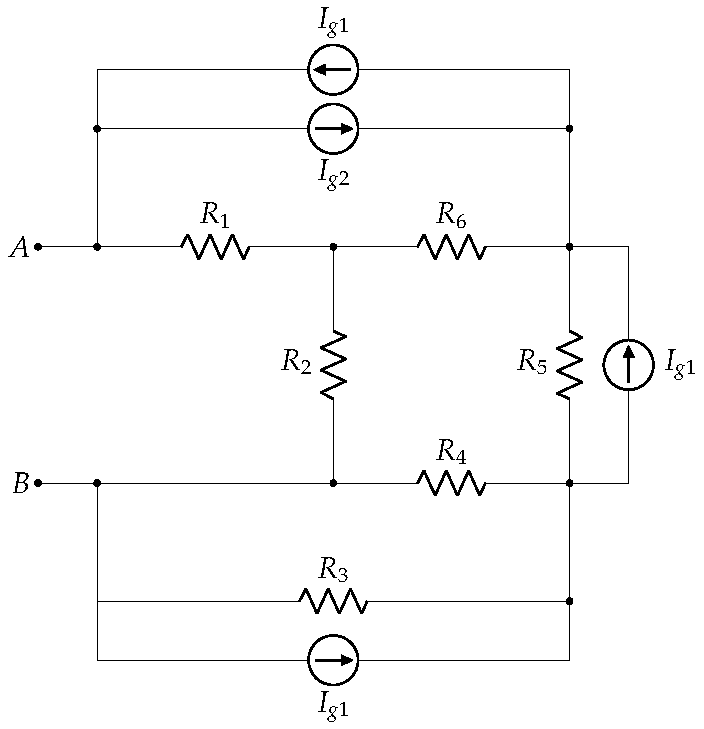
\includegraphics[height = 0.4\textheight]{figs/movilidad1.pdf}  
\end{center}

En este circuito, las fuentes $I_{g1}$ e $I_{g2}$ se cancelan mutuamente. Además, $R_3$ y $R_4$ están en paralelo. Representando este paralelo con $R_{34}$ obtenemos el siguiente circuito, en el que las fuentes de corriente han sido transformadas a fuentes de tensión.

\begin{center}
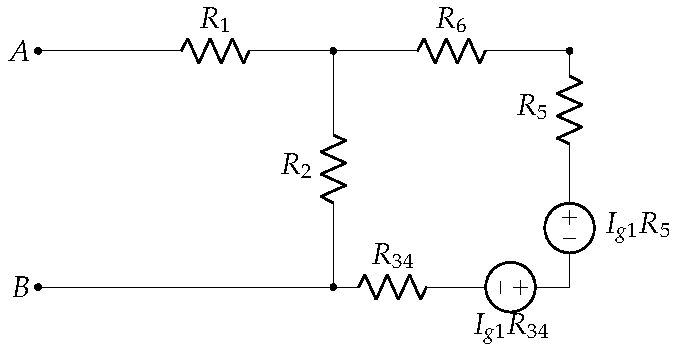
\includegraphics[height = 0.2\textheight]{figs/movilidad2.pdf}
\end{center}


A continuación, asociamos las resistencias $R_6$, $R_5$ y $R_{34}$, y las fuentes de tensión.

\begin{center}
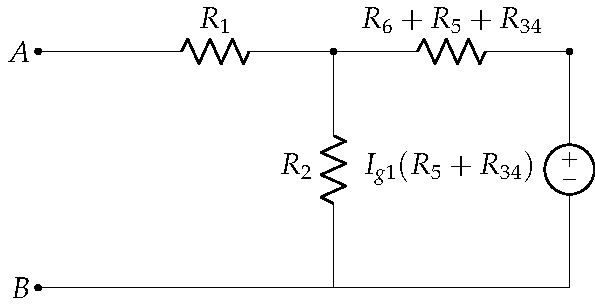
\includegraphics[height = 0.2\textheight]{figs/movilidad3.pdf}
\end{center}
A continuación, transformamos esta fuente de tensión en fuente de corriente, y asociamos las resistencias en paralelo. Nuevamente transformamos a fuente de tensión para obtener el generador equivalente de la figura:

\begin{center}
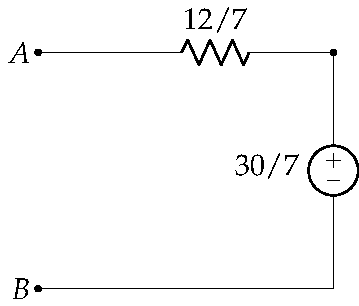
\includegraphics[height = 0.2\textheight]{figs/generadorEquivalente.pdf}
\end{center}



\clearpage 

\section{Sistemas Trifásicos}

El circuito trifásico de la figura trabaja a una tensión de \SI{300}{\volt} y con secuencia de fases inversa. El motor tiene una potencia de \SI[parse-numbers=false]{1.5\sqrt{3}}{CV}, factor de potencia de 0,8 y rendimiento del 92\%. La carga en estrella tiene los valores $X_c = X_L = R = \SI[parse-numbers = false]{20\sqrt{3}}{\ohm}$.

Debes determinar:\vspace{0.5cm}

\begin{minipage}{0.45\textwidth}
\begin{enumerate}
\item Las intensidades que miden los amperímetros.
\item Potencia activa, reactiva y aparente del conjunto.
\item Lectura de los vatímetros $W_a$ y $W_b$.
\item Justifica la relación entre la medida de los vatímetros y el triángulo de potencias del sistema.
\item Si se producen sendas roturas en los puntos indicados con asteriscos, determina las nuevas lecturas de los aparatos de medida.
\end{enumerate}
\end{minipage}
\begin{minipage}{0.55\textwidth}
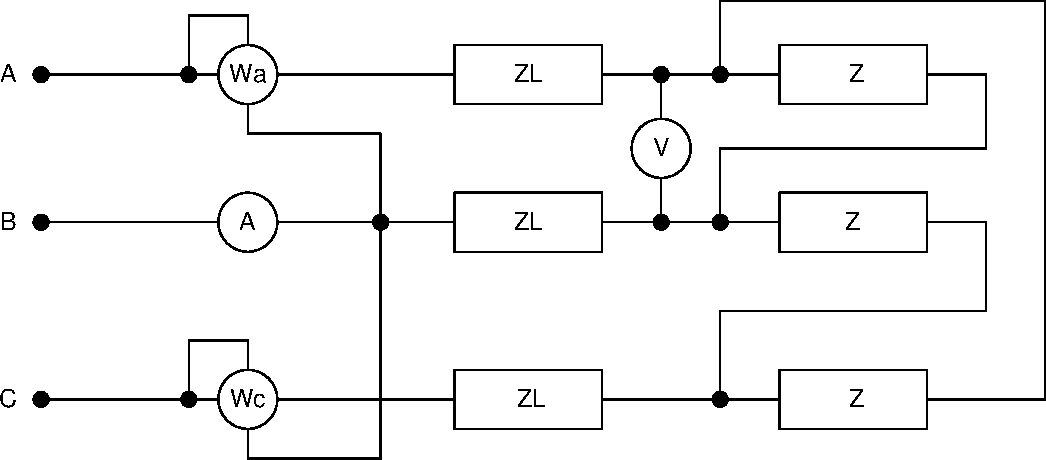
\includegraphics[width=\textwidth]{figs/trifasica.png}
\end{minipage}

\subsection*{Solución}

\includepdf[pages=-]{Solucion_Trifasica.pdf}

\clearpage

\section{Técnicas generales de análisis}

\begin{minipage}{0.5\textwidth}
  Determina las corrientes de todas las ramas del circuito resolviendo
  mediante el método de mallas.

  Datos:

  $i_g(t) = \sen(\omega t + \pi)$

  $\epsilon_g(t) = \cos(\omega t)$

  $\overline{Z}_1 = j\si{\ohm}$

  $\overline{Z}_2 = -j\si{\ohm}$

  $\overline{Z}_3 = \overline{Z}_4 = \SI{1}{\ohm}$

  $\alpha = \SI{1}{\ohm}$
\end{minipage}
\begin{minipage}{0.5\textwidth}
  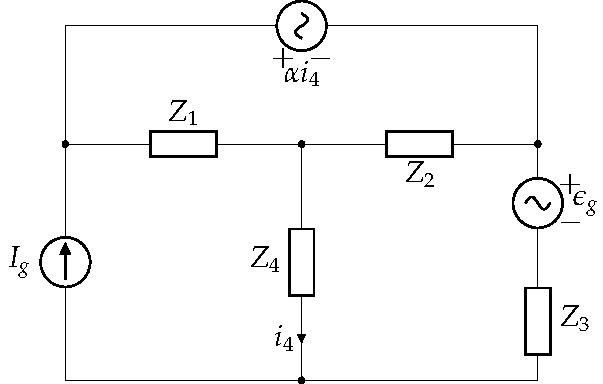
\includegraphics[width=\textwidth]{figs/mallas.pdf}
\end{minipage}

\subsection*{Solución}

En primer lugar, los fasores de las fuentes independientes son:

\begin{align*}
  \overline{I}_g = \frac{\sqrt{2}}{2}\phase{\pi}\\
   \overline{\epsilon}_g = \frac{\sqrt{2}}{2}\phase{\pi/2}\\
\end{align*}

Definimos las corrientes de malla y las corrientes de rama:

\begin{center}
  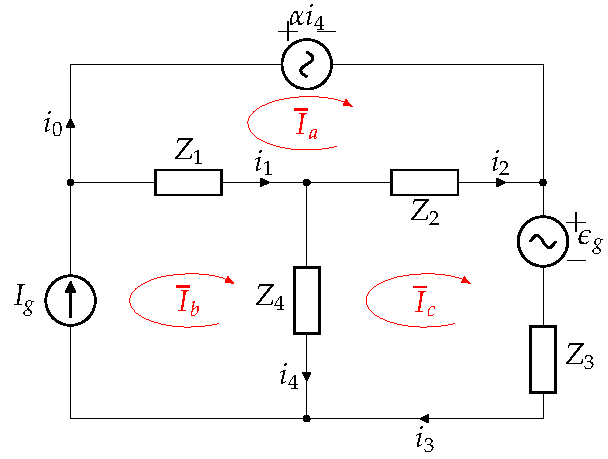
\includegraphics[height = 0.3\textheight]{figs/mallas_corrientes.pdf}
\end{center}

La ecuación de la malla A es:

\[
  (\overline{Z}_1 + \overline{Z}_2) \overline{I}_a - \overline{Z}_1 \overline{I}_g - \overline{Z}_2 \overline{I}_c = -\alpha \overline{I}_4
\]

La malla B está determinada por la fuente de corriente $\overline{I}_g$.

La ecuación de la malla C es:

\[
  - \overline{Z}_2 \overline{I}_a - \overline{Z}_4 \overline{I}_g + (\overline{Z}_2 + \overline{Z}_3 + \overline{Z}_4) \overline{I}_c = -\epsilon_g
\]

Además, la corriente de la que depende la fuente dependiente es:

\[
   \overline{I}_4 =  \overline{I}_g -  \overline{I}_c
 \]

 Sustituyendo valores en la ecuación de la malla A:


\[
  0 \cdot \overline{I}_a - j \cdot \overline{I}_g  + j \cdot \overline{I}_c = -\overline{I}_g + \overline{I}_c
\]

Despejamos $\overline{I}_c$:

\[
  \overline{I}_c = \overline{I}_g = \frac{\sqrt{2}}{2}\phase{\pi}
\]

Empleando este resultado en la ecuación de la malla C:

\[
  j \overline{I}_a - \overline{I}_g + (2 - j)\cdot \overline{I}_g = 
  - \overline{\epsilon}_g
\]

Despejamos $\overline{I}_a$:

\[
  \overline{I}_a = (1 + j)\cdot \overline{I}_g + j \overline{\epsilon}_g = (-2 - j) \frac{\sqrt{2}}{2}  = \SI[parse-numbers=false]{1.581\phase{\ang{-153.4}}}{\ampere}\\
\]

A partir de estos resultados obtenemos las corrientes de rama:

\begin{align*}
  \overline{I}_0 &= \overline{I}_a\\
  \overline{I}_1 &= \SI[parse-numbers=false]{1\phase{\ang{45}}}{\ampere}\\
  \overline{I}_2 &= \SI[parse-numbers=false]{1\phase{\ang{45}}}{\ampere}\\
  \overline{I}_3 &= \overline{I}_g\\
  \overline{I}_4 &= \SI{0}{\ampere}\\
\end{align*}

Por tanto,

\begin{align*}
  i_0(t) &= 2.236 \sen(\omega t -\ang{153.4})\\
  i_1(t) &= \sqrt{2} \sen(\omega t + \ang{45})\\
  i_2(t) &= \sqrt{2} \sen(\omega t + \ang{45})\\
  i_3(t) &= \sen(\omega t + \pi)\\
  i_4(t) &= 0
\end{align*}

\end{document}

% Local Variables:
% ispell-local-dictionary: "castellano"
% End:

